\documentclass[11pt,a4paper]{article}

\usepackage[T1]{fontenc}
\usepackage[utf8]{inputenc}
\usepackage{lmodern}
\usepackage[margin=2.3cm]{geometry}
\usepackage{microtype}
\usepackage{graphicx}
\usepackage{booktabs}
\usepackage{tabularx}
\usepackage[font=small,labelfont=bf]{caption}
\usepackage{float}
\usepackage{enumitem}
\usepackage{xcolor}
\usepackage[colorlinks=true,linkcolor=blue!50!black]{hyperref}

\graphicspath{{figures/}}
\setlist{nosep,leftmargin=*}
\setlength{\parskip}{0.5em}
\setlength{\parindent}{0pt}
\setlength{\emergencystretch}{3em}
\newcolumntype{Y}{>{\raggedright\arraybackslash}X}

\title{\textbf{IRWA Final Project --- Part 1}\\[0.2em]\large Text Processing and Exploratory Data Analysis}
\author{\begin{tabular}{ccc}Èric Amargant & Josep Cardona & Jan Balayla\\\small u231867 -- NIA 284566 & \small u231747 -- NIA 284888 & \small u233694 -- NIA 286572\end{tabular}}
\date{October 2026}

\begin{document}
\maketitle

The dataset contains \textbf{28,080 fashion products} from Flipkart. Our repository follows the course template.
All the Part~1 code is in \texttt{project\_progress/part\_1/}: the notebook \texttt{IRWA\_Part1.ipynb}, and the
cleaning functions in \texttt{irwa\_preprocessing.py}, which Part~2 will reuse to clean the queries the same way.

\textbf{GitHub repository:} \url{https://github.com/Janbacer/Final_Project_IRWA}\\
\textbf{Tag:} \texttt{IRWA-2026-part-1}\\
The \texttt{README.md} in the main folder of the repository explains step by step how to install the requirements
and run the code.

\section{Data preparation}

\subsection{Problems found in the data}
\begin{itemize}
  \item 40\% of the products have \textbf{no description}. Some fields are missing for a few percent of products:
        rating (8\%), brand (7\%) and seller (6\%).
  \item The text is messy: some words are glued together by punctuation (``look.Designed''), and ``T-shirt'' is
        written in 8 different ways (t-shirt, tshirt, t shirt, tee\ldots).
  \item \textbf{Brand names are cut off} (``Pu'' = Puma, ``REEB'' = Reebok). The product URL contains the full name,
        so we recover it from there. This works for 24,741 products.
  \item \textbf{Gender words disagree}: almost every URL says ``men'', while titles are half ``Men'' and half ``Women''.
        The validation labels follow the title (see 1.6), so we do not use the URL for search.
\end{itemize}

\subsection{Text pre-processing (point 1)}
Titles, descriptions and product details are cleaned with the same function, in this order:
\begin{enumerate}
  \item \textbf{Lowercase} the text.
  \item \textbf{Write a few fashion words in one way}: \texttt{t-shirt / t shirt / tee} $\to$ \texttt{tshirt},
        \texttt{sweat shirt} $\to$ \texttt{sweatshirt}, \texttt{polycotton} $\to$ \texttt{poly cotton},
        \texttt{slimfit} $\to$ \texttt{slim fit}. Without this, ``t-shirt'' would become ``t'' + ``shirt'', and every
        T-shirt would match the query ``shirt''.
  \item \textbf{Remove punctuation} by replacing it with spaces, which also separates glued words
        (``look.Designed'' $\to$ ``look designed'').
  \item \textbf{Tokenise} with \texttt{split()}, as in the lab sessions.
  \item \textbf{Remove stop words} (NLTK list). We keep \texttt{men} and \texttt{women} because they matter for relevance.
  \item \textbf{Remove numbers and one-letter tokens} (``100'', ``2'', ``s'').
  \item \textbf{Stem} with the Porter stemmer (as in the lab sessions) (\texttt{jeans} $\to$ \texttt{jean}, \texttt{printed} $\to$ \texttt{print}).
\end{enumerate}
\textbf{Example:} the query ``women full sleeve sweatshirt cotton'' becomes
\texttt{[women, full, sleev, sweatshirt, cotton]}. Over all titles and descriptions, the vocabulary goes from 10,606
words to 4,729 terms.

\subsection{Output fields (point 2)}
For every product we keep the \textbf{original fields unchanged}, so that search results can show them:
pid, title, description, brand, category, sub\_category, product\_details, seller, out\_of\_stock, selling\_price,
discount, actual\_price, average\_rating and url. Next to them we store the cleaned fields used for search. The
\texttt{pid} is never modified. The result is saved in \texttt{data/processed\_corpus.pkl}.

\subsection{Categorical fields (point 3)}
There were three options:
\begin{itemize}
  \item \textbf{Merge all fields into one text.} This is simple, but a match in the seller name then counts as much as a
        match in the title, and useless words make every document longer.
  \item \textbf{Keep each field separate.} Each field can get its own weight in the ranking, but there are more things to tune.
  \item \textbf{Use a field only as a filter.} This works well for exact choices (e.g.\ ``Footwear''), but the field
        never matches free-text queries.
\end{itemize}
A field only helps search if it is \textbf{distinctive}, i.e.\ if its values are not shared by most products.
We chose \textbf{separate fields}, plus one merged field for simple models:

\begin{table}[H]
\centering\small
\begin{tabularx}{\textwidth}{@{}l l Y@{}}
\toprule
field & decision & reason\\
\midrule
category & filter only & 96.6\% of the products have the same value, so it does not help separate them\\
sub\_category & text, low weight & only 24 broad values (``Topwear'', ``Bottomwear''), but on topic\\
brand & text, medium weight & very distinctive. But some brands are colour words (\emph{True Blue}, \emph{Black Beatle}),
which would wrongly match ``blue jeans'' if mixed with the main text\\
product\_details & text, high weight & contains what users search for: fabric, colour, sleeve, fit, gender.
We index the values only, and skip codes and boilerplate (Style Code, washing instructions\ldots)\\
seller & filter only & mostly repeats the brand, and users do not search by seller\\
\bottomrule
\end{tabularx}
\caption{How each categorical field is handled.}
\end{table}

\subsection{Numeric fields (point 4)}
\texttt{out\_of\_stock}, prices, discount and rating are \textbf{not indexed as text}: ``69\% off'' would become the
meaningless words ``69'' and ``off''. Instead we convert them to numbers (\texttt{"2,999"} $\to$ 2999). They can then
be used as \textbf{filters} (``under 1000'', ``in stock'') and as \textbf{ranking signals} (rating, discount).
A missing rating stays empty: it is not treated as a rating of 0.

\subsection{What the validation labels show}
Figure~\ref{fig:val} shows, for the labelled products, how many query terms appear in each field.
\begin{figure}[H]
\centering
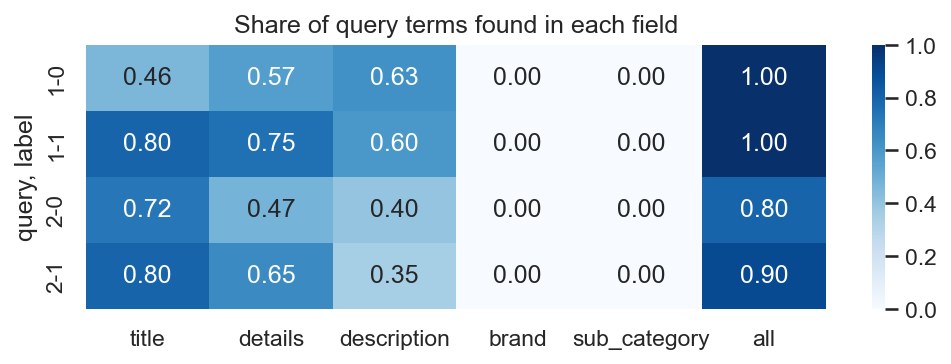
\includegraphics[width=0.7\textwidth]{validation_field_coverage.png}
\caption{Share of query terms found in each field (``1-0'' = query 1, not relevant).}
\label{fig:val}
\end{figure}
\begin{itemize}
  \item The \textbf{title} and the \textbf{product details} contain most query terms, and more of them for relevant
        products, so they should get the highest weights.
  \item \textbf{Gender matters}: for ``men slim jeans blue'', products with \emph{Men} in the title are relevant 78\% of
        the time, against 27\% for \emph{Women}. For query 1, T-shirts are never relevant.
  \item The \textbf{description} contains as many query terms for non-relevant products as for relevant ones,
        so it should get a low weight.
\end{itemize}

\section{Exploratory data analysis}

These analyses were chosen because they decide how to search in Part~2: which text fields carry useful terms, and which other values can filter or rank products when the text score is the same.
Named-entity recognition checks whether spaCy is a better source of brand names than the brand field.

\textbf{Categories.} Almost everything is clothing (96.6\%), and \emph{Topwear} alone is 55\% of the products.

\textbf{Text.} Titles are short: 6.9 words on average, following a fixed pattern
(``Printed Men Round Neck Black T-Shirt''). Descriptions have 50.9 words on average when present,
3.3 sentences per description, and an average sentence length of 15.5 words. After cleaning, the vocabulary has
6,343 terms. Titles are mostly about gender, product type and style. Descriptions add marketing words
(``comfort'', ``quality'', ``look'') that do not help search (Figure~\ref{fig:wc}).

\begin{figure}[H]
\centering
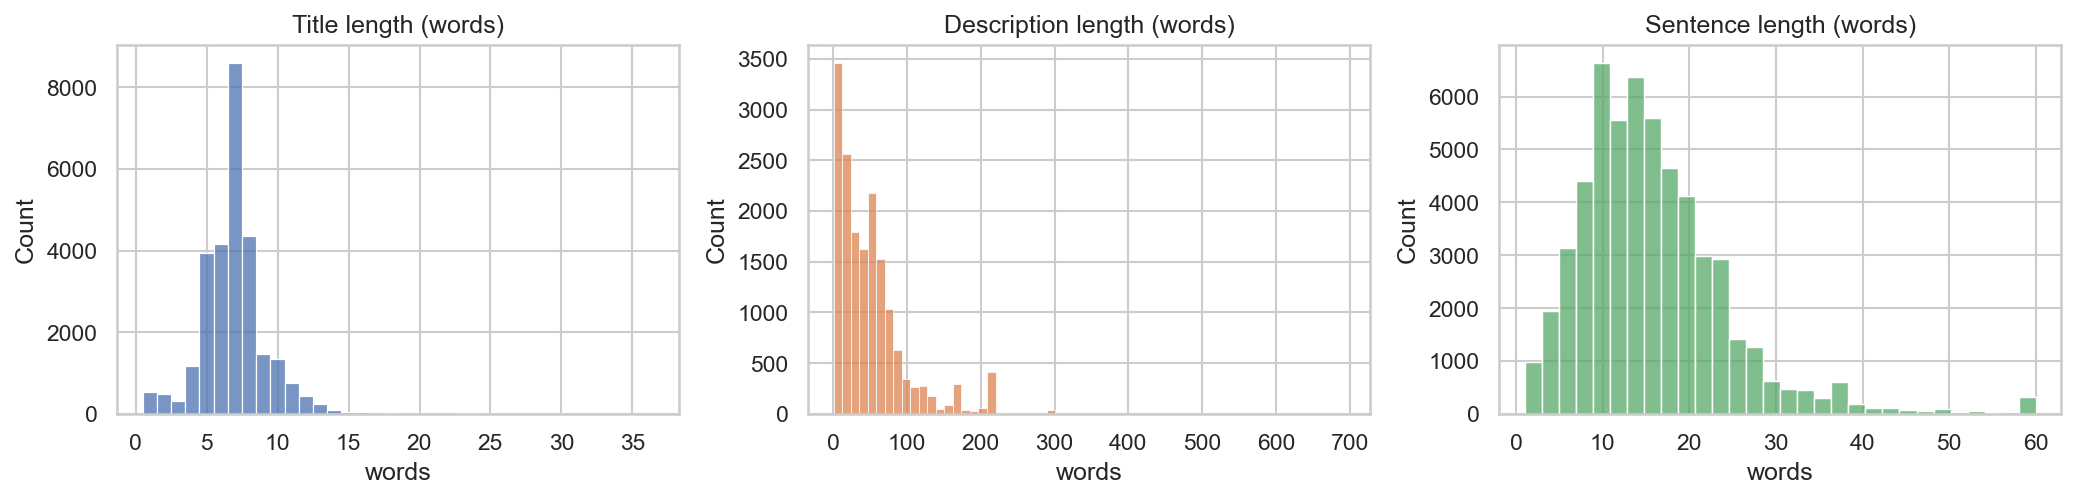
\includegraphics[width=\textwidth]{lengths.png}
\caption{Distribution of the number of words per title, per description and per sentence.}
\end{figure}

\begin{figure}[H]
\centering
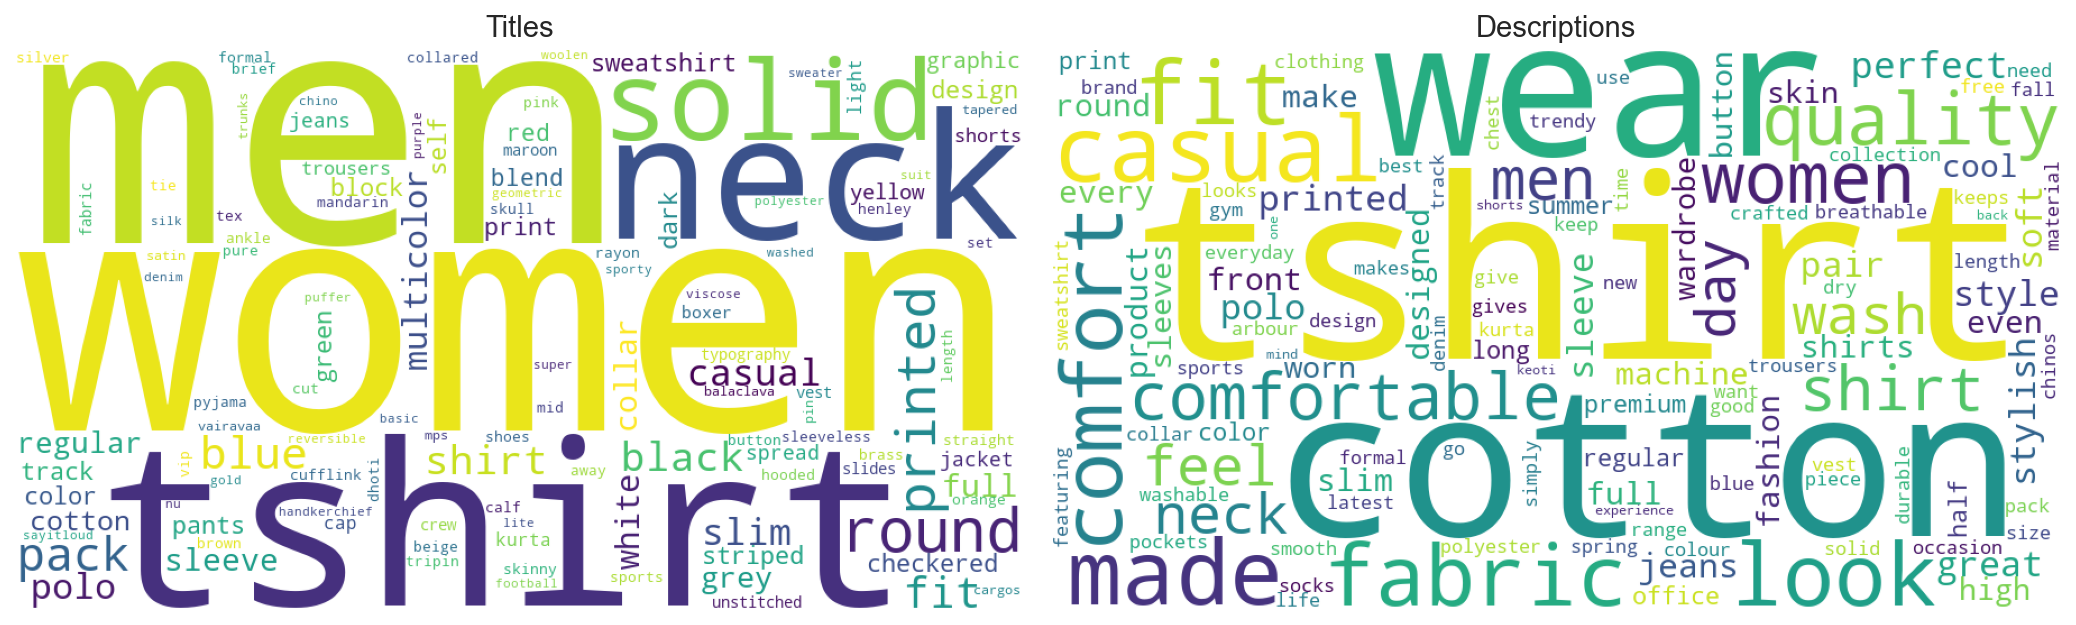
\includegraphics[width=\textwidth]{wordclouds.png}
\caption{Word clouds of the most frequent words in titles and descriptions.}
\label{fig:wc}
\end{figure}

\textbf{Prices, discounts and ratings.} Prices are low (median 545 rupees), discounts are large (median 53\%) and
ratings are mostly between 3.2 and 4.1 (Figure~\ref{fig:prices}). 329 products are rated 5.0, and there is no number
of reviews. For example, a 5.0 rating may come from a single review. Rating is therefore a weak signal.

\begin{figure}[H]
\centering
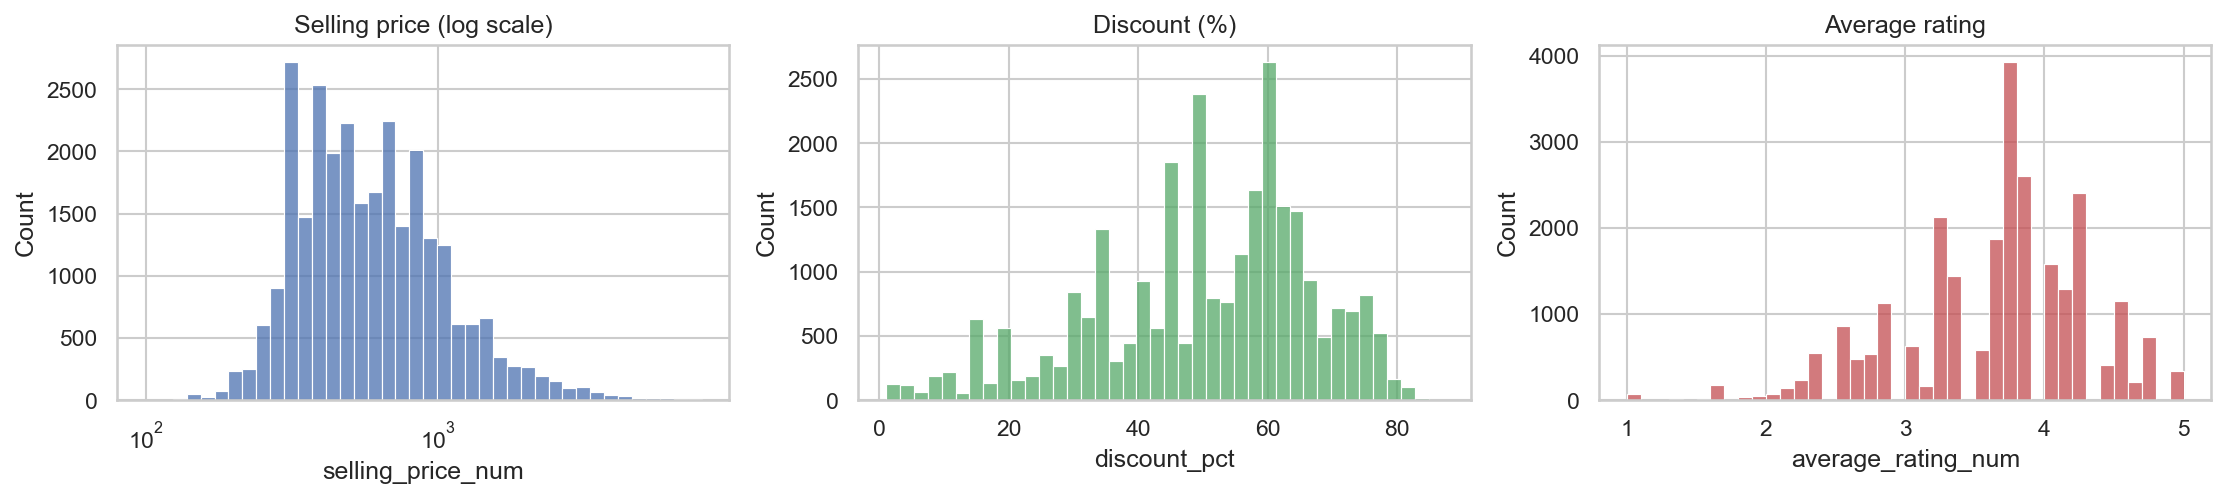
\includegraphics[width=\textwidth]{prices_ratings.png}
\caption{Distribution of selling price, discount and rating.}
\label{fig:prices}
\end{figure}

\textbf{Rankings.} 329 products tie for the highest rating (5.0).
Tables~\ref{tab:top-rating}--\ref{tab:top-price} list the top five by rating, by discount and by selling price.
The rating list breaks the tie by discount.
The brands with the most products are Ecko Unltd, Free Authority, Arbour, Reebok and Puma.
The largest seller is RetailNet (Figure~\ref{fig:brands}).

\begin{table}[H]
\centering\small
\begin{tabularx}{\textwidth}{@{}c Y l r r r@{}}
\toprule
 & title & brand & price & discount & rating\\
\midrule
1 & Men Solid Cotton Blend Pathani Kurta (Blue) & Purple State & 449 & 82\% & 5.0\\
2 & Printed Men Boxer (Pack of 1) & Sayitloud & 249 & 78\% & 5.0\\
3 & Printed Women Round Neck Multicolor T-Shirt & Yellowvibes & 275 & 77\% & 5.0\\
4 & Printed Women Round Neck Black T-Shirt & Pixfab & 289 & 77\% & 5.0\\
5 & Solid Women Round Neck Black T-Shirt & Pixfab & 288 & 77\% & 5.0\\
\bottomrule
\end{tabularx}
\caption{Top 5 products by rating. All are rated 5.0; the order uses discount to break the tie.}
\label{tab:top-rating}
\end{table}

\begin{table}[H]
\centering\small
\begin{tabularx}{\textwidth}{@{}c Y l r r r@{}}
\toprule
 & title & brand & price & discount & rating\\
\midrule
1 & Printed Women Round Neck White T-Shirt & Jack Royal & 128 & 87\% & 3.0\\
2 & Printed Women Round Neck Grey T-Shirt & Jack Royal & 136 & 86\% & 4.1\\
3 & Printed Women Round Neck White T-Shirt & Jack Royal & 136 & 86\% & 4.7\\
4 & Printed Men Round Neck Multicolor T-Shirt (Pack of 2) & Yellowvibes & 449 & 85\% & 3.2\\
5 & Solid Balclava Cap & Graceway & 228 & 84\% & 4.3\\
\bottomrule
\end{tabularx}
\caption{Top 5 products by discount. Price is the selling price in rupees.}
\label{tab:top-discount}
\end{table}

\begin{table}[H]
\centering\small
\begin{tabularx}{\textwidth}{@{}c Y l r r r@{}}
\toprule
 & title & brand & price & discount & rating\\
\midrule
1 & Solid Women Track Suit & Reebok & 7,999 & 20\% & 2.7\\
2 & Checkered Single Breasted Party Women Full Sleeve Blazer (Grey) & True Blue & 7,998 & --- & 2.6\\
3 & Full Sleeve Solid Women Casual Jacket & Puma & 7,799 & 40\% & 3.7\\
4 & Full Sleeve Printed Men Sweatshirt & Puma & 7,799 & 40\% & 4.5\\
5 & Skinny Men Blue Jeans & Gas & 7,794 & 40\% & 4.2\\
\bottomrule
\end{tabularx}
\caption{Top 5 products by selling price, in rupees. The True Blue blazer has no discount.}
\label{tab:top-price}
\end{table}

\begin{figure}[H]
\centering
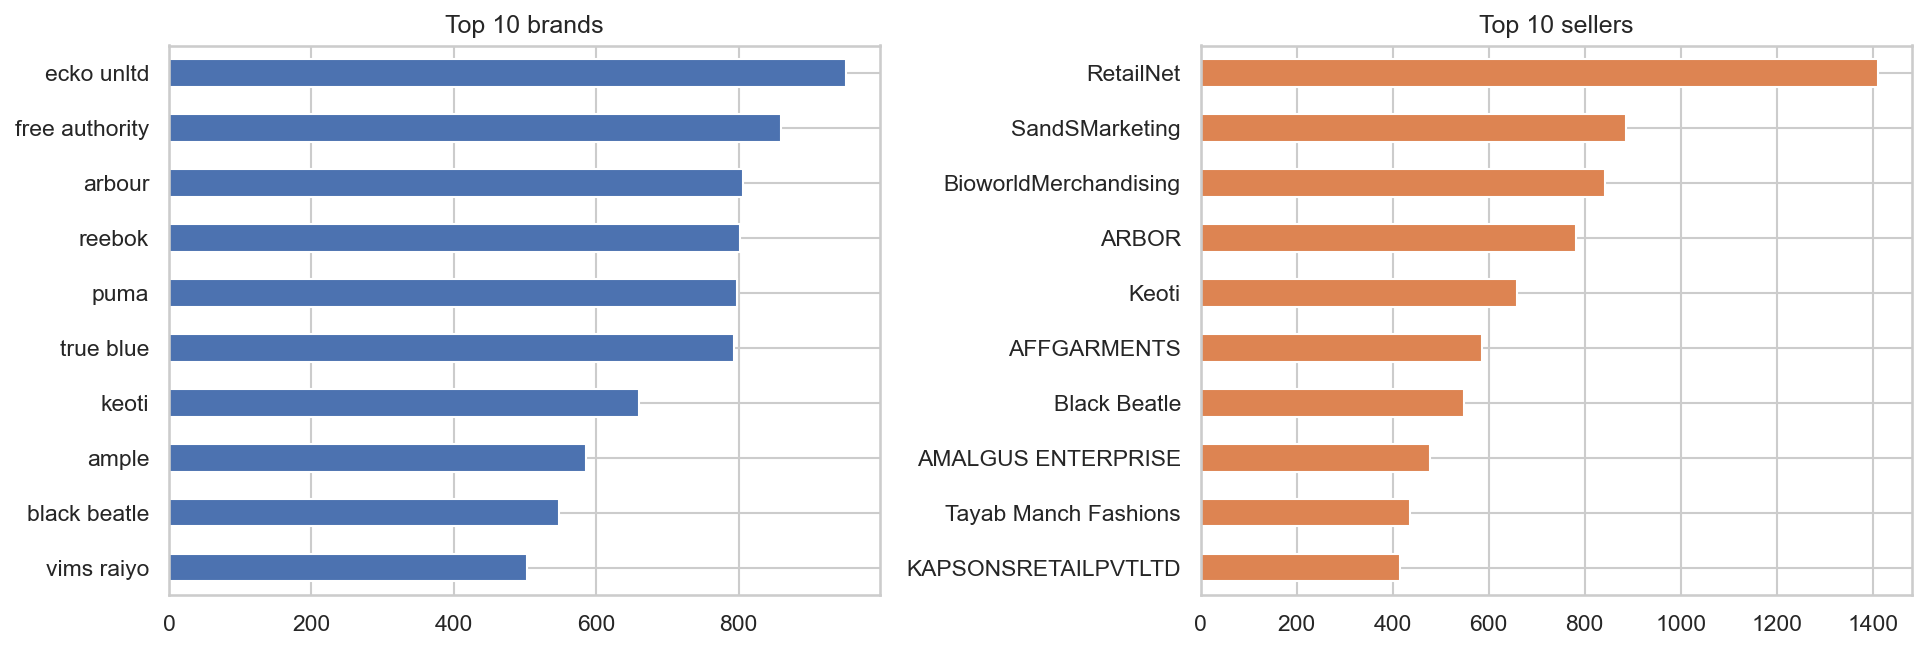
\includegraphics[width=0.9\textwidth]{brands_sellers.png}
\caption{Top brands and sellers by number of products.}
\label{fig:brands}
\end{figure}

\textbf{Stock.} 5.9\% of the products (1,644) are out of stock. The rate is highest in Clothing Accessories and Tracksuits
(Figure~\ref{fig:stock}).

\begin{figure}[H]
\centering
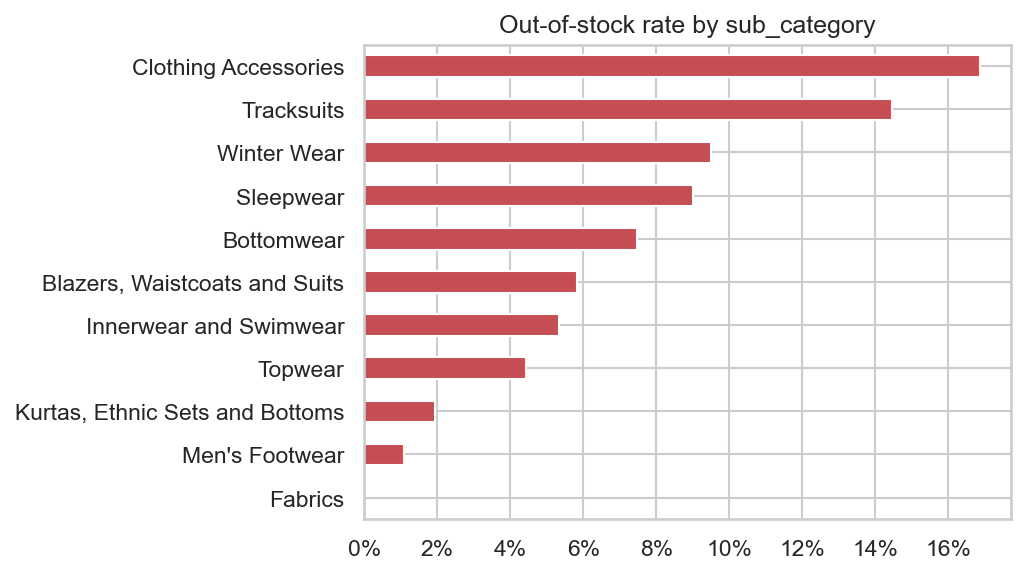
\includegraphics[width=0.75\textwidth]{out_of_stock.png}
\caption{Out-of-stock rate by subcategory.}
\label{fig:stock}
\end{figure}

\textbf{Duplicates.} 87\% of the products share their title with another product. Most products are colour or size
variants of the same item, so many of them will get exactly the same text score in Part~2.

\textbf{Named entities.} spaCy finds some real brands (Reebok, Free Authority), but it makes many mistakes on product
text (Figure~\ref{fig:ner}). For example, it tags ``Cotton Blend Fabric'' as an organisation. The brand field is more reliable than NER.

\begin{figure}[H]
\centering
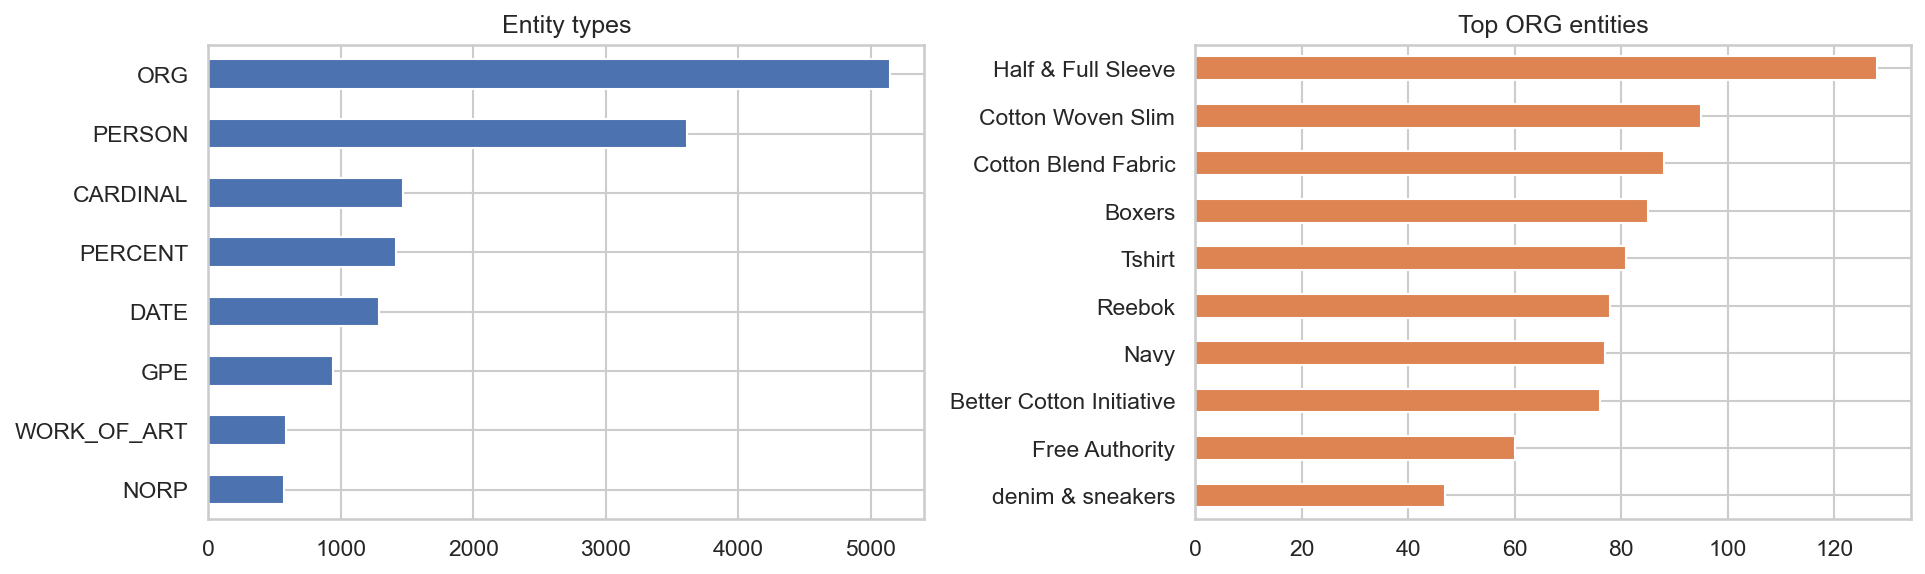
\includegraphics[width=\textwidth]{ner.png}
\caption{Entity types found by spaCy, and the most frequent organisation entities.}
\label{fig:ner}
\end{figure}

\section{Assumptions}
\begin{itemize}
  \item The title (and \texttt{product\_details}) give the correct gender of a product; the URL does not.
  \item The brand name at the start of the product URL is the full version of the truncated \texttt{brand} field.
  \item Missing prices or discounts (under 3\% of the products) are left empty; we do not try to guess them.
  \item A missing rating means ``not rated yet'', not a bad rating, so it is kept empty instead of 0.
  \item Numbers inside titles and descriptions (``100\% cotton'', ``pack of 2'') are not useful search terms.
\end{itemize}

\section{Conclusions for Part 2}
\begin{itemize}
  \item Clean documents and queries with the same function.
  \item Search mainly in the title and the product details, with lower weights for brand, sub\_category and description.
  \item Use category, seller, price, discount, rating and stock as filters or ranking signals, not as text.
\end{itemize}

\section*{Use of AI tools}
We used AI tools to revise grammar and improve the clarity of our writing, but not to develop or write the core theoretical concepts. In coding, we used AI to correct errors and refactor code, always starting from an initial implementation that we designed ourselves.
\end{document}
